\chapter{Descripci\'on del Corpus}\label{chapter:proposal}
En este cap\'itulo se propone un modelo de anotaci\'on de prop\'osito general de atributos protegidos
en textos. 
AQUI HAY QUE HACER UN PARRAFITO DESCRIBIENDO TODO LO QUE SE VA A HACER EN ESTE CAPITULO Y COMO SE VA A ORGANIZAR

\section{Esquema de anotaci\'on}\label{section:annotation_scheme}
%Hablar de que cada elemento a anotar es un texto, no una sola oracion.ok
%Hablar de cuales son los atributos protegidos que se anotaron. ok
%Hablar de los valores de cada atributo protegido y mas cosas relacionadas.ok/2
En el proceso de construcci\'on del corpus, cada elemento a anotar es un texto completo, puede estar formado por varias oraciones. 
Este enfoque permite capturar el contexto completo en el que se producen las menciones a los atributos protegidos, 
lo cual es importante para poder realizar un an\'alisis m\'as profundo de (decir algo aqui como que es mejor asi para tratar los sesgos).

En este caso, los atributos protegidos que se van a anotar son el g\'enero y la raza.
Fueron seleccionados estos atributos no solo por su relevancia en diversas \'areas de estudio y aplicaci\'on, sino tambi\'en 
por la naturaleza de los textos que se van a anotar. Dado que las rese\~nas de pel\'iculas y series de televisi\'on
pueden contener un amplia gama de discusiones sobre actores, directores y personajes, es muy probable que se haga menci\'on a 
estos atributos.

Para el atributo g\'enero los valores a anotar son: ``Male'' para g\'enero masculino, ``Female'' para g\'enero femenino, 
``Male, Female'' cuando se detectan ambos g\'eneros y ``Null'' en caso de no detectar ninguno.

En cuanto a la raza, los valores a anotar son: ``White'' para raza blanca, ``Black'' para raza negra, ``Indian'' para 
personas originarias de la India, ``Arab'' para personas de origen \'arabe, que incluye a pa\'ises del medio oriente y el norte de 
\'Africa. Adem\'as se incorpora el valor ``Latino'' para personas de origen latinoamericano, ``Native American'' para personas 
originarias de los pueblos nativos de Am\'erica del Norte y ``Asian'' para personas asi\'aticas. Al igual que con el g\'enero, 
``Null'' indica que no se detecta ninguna raza en el texto. N\'otese que, en caso de ser necesario la anotaci\'on de la raza de un 
texto puede incluir m\'as de un valor.

\section{Proceso de anotaci\'on}\label{section:annotation_process}
El proceso de anotaci\'on comienza con la selecci\'on de los textos a anotar. Inicialmente se contaba con un conjunto de 70 textos 
extra\'idos de rese\~nas de pel\'iculas de ImDb\footnote{\url{https://www.imdb.com/}}, previamente anotados con g\'enero, producto 
de una tesis del grupo de investigaci\'on. A esta selecci\'on se a\~naden 80 textos m\'as extra\'idos de la misma fuente, con el 
objetivo de aumentar el tama\~no y la diversidad del corpus. Los nuevos textos se seleccionan de manera aleatoria.

Una vez seleccionados los textos, se procede a la anotaci\'on de los atributos protegidos. Esta etapa se divide en tres fases 
fundamentales:

\begin{enumerate}
    \item Anotaci\'on exhaustiva de ambos atributos protegidos por parte de dos anotadores no expertos en la prolem\'tica. 
    Generando as\'i dos anotaciones independientes. Los anotadores tienen permitido intercambiar opiniones y consultar dudas
    con un anotador experto, pero no deben discutir las oraciones espec\'ificas que anotan.
    \item Mezcla de las anotaciones independientes. En caso de detectarse conflicto, un anotador experto se encarga de escoger la 
    anotaci\'on m\'as acertada. Esta etapa puede ser asistida por \emph{scripts} de mezcla que detecten y resalten autom\'aticamente
    los conflictos.
    \item Revisi\'on del resultado final por parte de un anotador experto, en busca de posibles errores e inconsistencias.
\end{enumerate}

Luego de estas tres fases, el conjunto de textos resultante de mezclar y revisar ambas anotaciones manuales constituye el corpus, el 
cual debe ser evaluado como se describe en la secci\'on~\ref{subsection:annotation_evaluation}.

\subsection{Evaluaci\'on de la anotaci\'on}\label{subsection:annotation_evaluation}
Se sugiere calcular un \emph{micro-agreement} y un \emph{macro-agreement} para evaluar el grado de concordancia entre las anotaciones
manuales del corpus. Adem\'as, se propone estudiar la consistencia estad\'istica de las anotaciones, mediante el c\'alculo  
de media, varianza y desviaci\'on est\'andar de los acuerdos entre anotadores, para cada atributo protegido.
%#TODO: Ver como disminuir el uso de la palabra anotadores, anotaciones...

La comparaci\'on anterior puede ser realizada en dos fases. En la primera fase, se realiza la comparaci\'on entre las anotaciones 
realizadas por los anotadores no expertos. Luego, en la segunda fase, se realiza la comparaci\'on entre las anotaciones de los 
anotadores no expertos y el resultado de la mezcla y revisi\'on por parte del anotador experto. En la secci\'on~\ref{section:results} 
se muestran los resultados obtenidos en la evaluaci\'on del corpus.

Primero se define una m\'etrica $\mathcal{J}_{attr}(A, B) \in [0,1]$, conocida como \emph{coeficiente de Jaccard}. Dicha m\'etrica 
determina para un texto el grado de concordancia entre sus dos anotaciones $A$ y $B$ de un atributo protegido $attr$, adem\'as 
considera coincidencia parcial entre las anotaciones. Se calcula:

\begin{equation*}
    \mathcal{J}_{attr}(A, B) = \frac{|A \cap B|}{|A \cup B|} = \begin{cases}
        1, & \text{si coinciden ex\'actamente} \\
        0, & \text{si la intersecci\'on es vac\'ia} \\
        0 < p < 1, & \text{en otro caso}
    \end{cases}
\end{equation*}

Se define el conjunto $C_{attr} = \{\mathcal{J}_{attr}(A, B) \mid \forall (A, B)\}$. Para analizar la consistencia estad\'istica 
de las anotaciones, se calcula la media, varianza y desviaci\'on est\'andar de los conjuntos $C_{g\acute{e}nero}$ y $C_{raza}$.

%#TODO: Pedirle al profe que se lea este parrafo a ver si queda claro lo que se propone en el
Para calcular el \emph{micro-agreement}, se realiza la uni\'on de las anotaciones de ambos atributos protegidos, obteniendo as\'i
el conjunto $C_{g\acute{e}nero, raza} = \{\mathcal{J}_{attr}(A, B) \mid \forall (A, B)\}$. Luego, se calcula la media, varianza y
desviaci\'on est\'andar del conjunto obtenido. Estos resultados son una medida detallada de la concordancia en t\'erminos puntuales.
Se muestran en la secci\'on~\ref{section:results}.

Por otra parte, la m\'etrica \emph{macro-agreement} se calcula como la media de los \emph{micro-agreements} de cada atributo protegido. 
Esta m\'etrica ofrece una perspectiva m\'as general de la concordancia entre las anotaciones. Se muestran en la 
secci\'on~\ref{section:results}.

\subsection{Directrices de anotaci\'on}\label{section:annotation_guidelines}
%Hablar que para anotar cierto atributo no hacer falta que el texto lo mencione explicitamente, sino que se puede inferir
%Ejemplo las entidades nombradas
La caracter\'istica m\'as importante de este modelo de anotaci\'on es que busca capturar cualquier tipo de referencia a los atributos 
protegidos que se anotan. Por lo tanto, la anotaci\'on no se limita \'unicamente a menciones expl\'icitas de estos atributos en el 
texto, sino que tambi\'en se extiende a situaciones donde la referencia a g\'enero y raza puede ser inferida. La inferencia puede 
basarse en diversos elementos del texto, por ejemplo, entidades nombradas y pronombres. En caso de ser necesario el anotador podr\'a
auxiliarse de informaci\'on externa, como la b\'usqueda de im\'agenes de los personajes mencionados en el texto.

\subsection{Herramientas de anotaci\'on}
%Describir los scripts que se hicieron para anotar, mezclar y todo eso
Se desarrollaron dos \emph{scripts} de \emph{Python} para asistir en el proceso de anotaci\'on. Un primer \emph{script}
se encarga de guiar al anotador en todo este proceso, mostrando los textos a anotar y permitiendo la selecci\'on de los valores
que correspondana a cada atributo protegido. Adem\'as, este \emph{script} almacena continuamente las anotaciones en un archivo
\emph{CSV}, para evitar p\'erdidas de informaci\'on en caso de que ocurra alg\'un error. El segundo \emph{script} se encarga de
mezclar las anotaciones de los anotadores no expertos, resaltando los conflictos y permitiendo la selecci\'on de la anotaci\'on
m\'as acertada por parte del experto. Este \emph{script} tambi\'en almacena las anotaciones en un archivo nuevo archivo
\emph{CSV}.

\section{Estad\'isticas del Corpus}
El corpus fue construido a partir un fichero \emph{CSV}, tomado de la plataforma 
Kaggle\footnote{\url{https://www.kaggle.com/datasets/mantri7/imdb-movie-reviews-dataset}}. 
Este fichero contiene 24904 rese\~nas de pel\'iculas en idioma espa\~nol. Cada entrada del fichero contiene el texto de la rese\~na, 
y un atributo binario anotado que indica si la rese\~na es positiva o negativa. Se contaba inicialmente con un conjunto de 70 textos 
preseleccionados, a los que se a\~nadieron 80 nuevos textos seleccionados de manera aleatoria.

Usando este conjunto de textos, se implement\'o un proceso de anotaci\'on para etiquetar manualmente el g\'enero y la raza seg\'un 
el modelo descrito en la secci\'on~\ref{section:annotation_scheme}. Este proceso de anotaci\'on se describe en detalle en la 
secci\'on~\ref{section:annotation_process}. La figura~\ref{fig:ann_proc} ilustra el procesamiento realizado.
Luego del proceso de anotaci\'on, se obtuvo un total de 150 textos anotados con g\'enero, raza y sentimiento, que constituyen el 
corpus final. Las tablas~\ref{table:stats},~\ref{table:stats_gen} y~\ref{table:stats_race}  resumen las estad\'isticas fundamentales 
del corpus final.

\begin{figure}[htpb]
    \begin{center}
        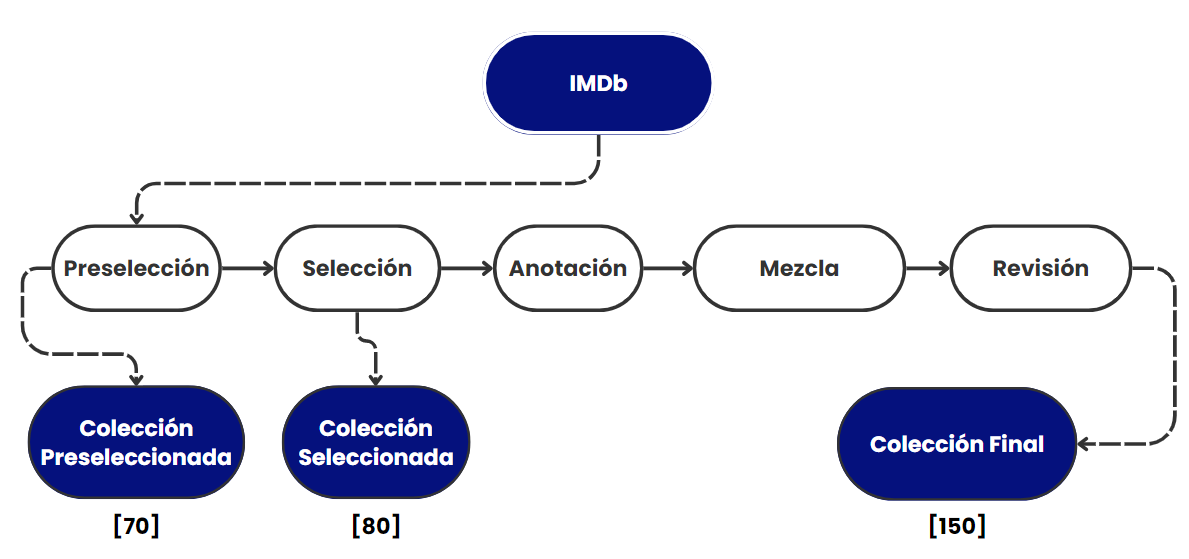
\includegraphics[width=0.8\textwidth]{Graphics/annotation_proc.png}
    \end{center}
    \caption{Representaci\'on esquem\'atica del proceso de anotaci\'on.}
    \label{fig:ann_proc}
\end{figure}

\begin{table}[htpb]
    \centering
        \begin{tabular}{lc}
        \toprule
        \textbf{M\'etrica} & \textbf{Total} \\
        \midrule
                    Textos & 150 \\
          G\'enero Anotado & 122 \\
              Raza Anotada & 107 \\

        \bottomrule
        \end{tabular}
    \caption{Resumen de las estad\'isticas generales del corpus: cantidad de textos, cantidad de textos con g\'enero anotado y 
    cantidad de textos con raza anotada.}
    \label{table:stats}
\end{table}

\begin{table}[htpb]
    \centering
        \begin{tabular}{lc}
        \toprule
          \textbf{Clase} & \textbf{Total} \\
        \midrule
                    Male & 102 \\
                  Female & 83 \\

        \bottomrule
        \end{tabular}
    \caption{Resumen de las estad\'isticas del corpus relacionadas con el atributo g\'enero: cantidad de textos por g\'enero.}
    \label{table:stats_gen}
\end{table}

\begin{table}[htpb]
    \centering
        \begin{tabular}{lc}
        \toprule
            \textbf{Clase} & \textbf{Total} \\
        \midrule
                     White & 87 \\
                     Black & 17 \\
                     Asian & 7 \\
                    Latino & 6 \\
                    Indian & 6 \\
                      Arab & 2 \\
           Native American & 1 \\

        \bottomrule
        \end{tabular}
    \caption{Resumen de las estad\'isticas del corpus, relacionadas con el atributo raza: cantidad de textos por raza.}
    \label{table:stats_race}
\end{table}

\section{Baseline}

\subsection{Detalles de implementaci\'on}

